\subsubsection{UC\theuccount-GP - Aggiunta nuovo utente}
		\begin{figure}[H]
			\centering
				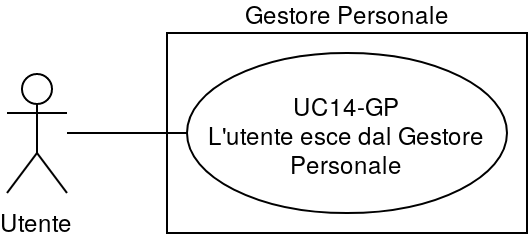
\includegraphics[width=\columnwidth]{img/casi_d'uso/UC14.png}\\
			\caption{UC\theuccount-GP - Aggiunta nuovo utente}
		\end{figure}
	\begin{itemize}
		\item \textbf{Codice}: UC\theuccount-GP.
		\item \textbf{Titolo}: aggiunta nuovo utente.
		\item \textbf{Attori primari}: utente.
		\item \textbf{Descrizione}: l'utente, acceduto al sistema, aggiunge un nuovo utente nel sistema.
		Non è possibile che un utente non acceduto si iscriva da solo per la prima volta.
		\item \textbf{Precondizione}: un nuovo utente deve essere aggiunto nel sistema.
		\item \textbf{Postcondizione}: un utente viene aggiunto al sistema.
		\item \textbf{Scenario principale}:
		\begin{enumerate}
			\item L'utente aggiunge un nuovo utente
		\end{enumerate}
	\end{itemize}

	\stepcounter{subuccount}
	\subsubsection{UC\theuccount.\thesubuccount-GP - Utente aggiunto con successo}
		\begin{figure}[H]
			\centering
			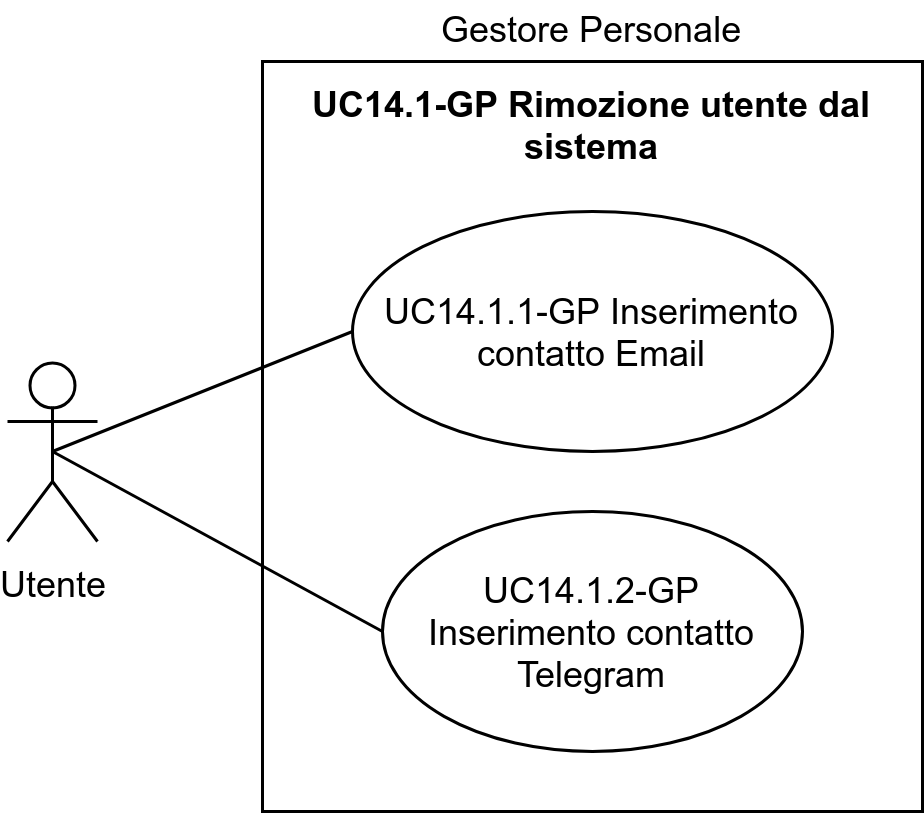
\includegraphics[width=\columnwidth]{img/casi_d'uso/UC14_1.png}\\
			\caption{UC\theuccount.\thesubuccount-GP - Utente aggiunto con successo}
		\end{figure}
		\begin{itemize}
			\item \textbf{Codice}: C\theuccount.\thesubuccount-GP.
			\item \textbf{Titolo}: utente aggiunto con successo.
			\item \textbf{Attori primari}: utente.
			% non acceduto.
			\item \textbf{Descrizione}: un nuovo utente viene inserito con successo nel sistema.
			\item \textbf{Precondizione}: un nuovo utente deve essere aggiunto nel sistema.
			\item \textbf{Postcondizione}: un utente viene aggiunto con successo al sistema.
			\item \textbf{Scenario principale}:
			\begin{enumerate}
				\item L'utente inserisce i dati del nuovo utente da aggiungere
				\item L'utente conferma l'invio dei dati
				\item L'aggiunta viene effettuata con successo
			\end{enumerate}
			\item \textbf{Estensioni}:
			\begin{itemize}
				\item Errore utente già presente nel sistema [UC\theuccount.2-GP]
			\end{itemize}
		\end{itemize}
		
		\stepcounter{subsubuccount}
		\subsubsection{UC\theuccount.\thesubuccount.\thesubsubuccount-GP - Inserimento nome utente}
			
			\begin{itemize}
				\item \textbf{Codice}: UC\theuccount.\thesubuccount.\thesubsubuccount-GP.
				\item \textbf{Titolo}: inserimento nome utente.
				\item \textbf{Attori primari}: utente.
				%non registrato.
				\item \textbf{Descrizione}: l'utente inserisce il nominativo dell'utente da aggiungere.
				\item \textbf{Precondizione}: un nuovo utente deve essere aggiunto nel sistema.
				\item \textbf{Postcondizione}: il nome del nuovo utente è stato aggiunto nel sistema.
				\item \textbf{Scenario principale}:
				\begin{enumerate}
					\item L'utente aggiunge il nominativo del nuovo utente
				\end{enumerate}
			\end{itemize}
		
		\stepcounter{subsubuccount}
		\subsubsection{UC\theuccount.\thesubuccount.\thesubsubuccount-GP - Inserimento cognome utente}
			
			\begin{itemize}
				\item \textbf{Codice}: UC\theuccount.\thesubuccount.\thesubsubuccount-GP.
				\item \textbf{Titolo}: inserimento cognome utente.
				\item \textbf{Attori primari}: utente.
				% non registrato.
				\item \textbf{Descrizione}: l'utente inserisce il cognome dell'utente da aggiungere.
				\item \textbf{Precondizione}: un nuovo utente deve essere aggiunto nel sistema.
				\item \textbf{Postcondizione}: il cognome del nuovo utente è stato aggiunto nel sistema.
				\item \textbf{Scenario principale}:
				\begin{enumerate}
					\item L'utente aggiunge il cognome del nuovo utente
				\end{enumerate}
			\end{itemize}
		
		\stepcounter{subsubuccount}
		\subsubsection{UC\theuccount.\thesubuccount.\thesubsubuccount-GP - Inserimento contatto Email}
			
			\begin{itemize}
				\item \textbf{Codice}: UC\theuccount.\thesubuccount.\thesubsubuccount-GP.
				\item \textbf{Titolo}: inserimento contatto Email.
				\item \textbf{Attori primari}: utente.
				% non registrato.
				\item \textbf{Descrizione}: l'utente inserisce il contatto Email dell'utente da aggiungere.
				\item \textbf{Precondizione}: un nuovo utente deve essere aggiunto nel sistema.
				\item \textbf{Postcondizione}: il contatto Email è stato aggiunto.
				\item \textbf{Scenario principale}:
				\begin{enumerate}
					\item L'utente aggiunge il contatto Email del nuovo utente
				\end{enumerate}
		\end{itemize}
		
		\stepcounter{subsubuccount}
		\subsubsection{UC\theuccount.\thesubuccount.\thesubsubuccount-GP - Inserimento contatto Telegram}
			
			\begin{itemize}
				\item \textbf{Codice}: UC\theuccount.\thesubuccount.\thesubsubuccount-GP.
				\item \textbf{Titolo}: inserimento contatto Telegram.
				\item \textbf{Attori primari}: utente.
				% non registrato.
				\item \textbf{Descrizione}: l'utente inserisce il contatto Telegram dell'utente da aggiungere.
				\item \textbf{Precondizione}: un nuovo utente deve essere aggiunto nel sistema.
				\item \textbf{Postcondizione}: il contatto Telegram è stato aggiunto.
				\item \textbf{Scenario principale}:
				\begin{enumerate}
					\item L'utente aggiunge il contatto Telegram del nuovo utente
				\end{enumerate}
			\end{itemize}
	
	\stepcounter{subuccount}
	\subsubsection{UC\theuccount.\thesubuccount-GP - Errore utente già presente nel sistema}
		
		\begin{itemize}
			\item \textbf{Codice}: UC\theuccount.\thesubuccount-GP.
			\item \textbf{Titolo}: errore utente già presente nel sistema.
			\item \textbf{Attori primari}: utente.
			\item \textbf{Descrizione}: l’utente viene avvisato che i contatti Telegram o Email immessi non sono univoci.
			\item \textbf{Precondizione}: un nuovo utente deve essere aggiunto nel sistema.
			\item \textbf{Postcondizione}: il sistema comunica all’utilizzatore l’errore e l'utente non viene inserito.
			\item \textbf{Scenario principale}:
			\begin{enumerate}
				\item L'utente visualizza il messaggio d'errore
			\end{enumerate}
			\end{itemize}